%%%%%%%%%%%%%%%%%%%%%%%%%%%%%%%%%%%
\subsection{Thermometers}
\label{sec:fdsp-slow-cryo-therm}
% anselmo, jelena,

As mentioned above, a detailed 3D temperature map is important to monitor the correct functioning of the cryogenic system and the LAr uniformity.
Given the complexity and size of purity monitors, those can only be installed on the cryostat sides to provide a local measurement of
the LAr purity. While a direct measurement of the LAr purity across the entire cryostat is not realistic, a sufficiently detailed 3D temperature map
can be used to predict the LAr purity using CFD simulations. Specially important is the vertical coordinate since this will be closely related to
the LAr flow and uniformity. 

High precision temperature sensors will be distributed near the TPC walls in two ways:
i) forming high density (>1 sensor/m) vertical arrays (the so-called T-gradient monitors), and ii) in coarser ($~$ 1 sensor/5 m) 2D arrays 
at the top and bottom of the detector, which are the most delicate regions (the so-called individual sensors).   

Since temperature variations inside the cryostat are expected to be very small ($0.02 K$), to properly measure the 3D temperature map 
sensors must be cross-calibrated to better than $0.005 K$. Most sensors will be calibrated in the laboratory, prior to installation,
as described in the next section. This is in fact the only viable method for sensors behind the APAs and top/bottom of the detector since the available space is restricted.  
Given the precision required and the unknown longevity of the sensors (which could require a new calibration after sometime), and complementary method
will be used for T-gradient monitors behind the front end-walls. In those areas there is sufficient space for a movable system, which can be used to cross-calibrate insitu
the temperature sensors. This calibration method is described in the section about dynamic T-gradient monitors. 

In the baseline design for all three systems mentioned above three elements are common: the sensor model, the cable model and the readout system.
The baseline sensor model is the Lakeshore PT102, which has demonstrated excelent performance in ProtoDUNE-SP. Those sensors have  ...
For the readout cables a custom cable made by Axon is the baseline. It consists in four teflon-jacketed (extruded PFA)
silver platted annealed cupper wires (AWG28), forming two twisted pairs, with an metalic external shield
(silver platted annealed cupper) and an outer teflon (extruded PFA) jacket. The cable has a 3.7 mm outer diameter and weights 28 g/m.
The redout system will be descrived below in a separate subsection. 

% % % %
\subsubsection{Static T-Gradient monitors}

Several vertical arrays of high precision temperature sensors cross-calibrated in the laboratory will be installed behind the APAs.
Since the electric potential in this area is zero no electric field shielding is required, simplifying enormously the mechanical design.

Sensors are cross-calibrated in the lab using a well controlled environment and a high precission readout system, descrived below in a separate subsection.  
Four sensors are placed as close as possible in a small cylyndrical aluminum capsule. The capsule is introduced in a polystire box with 15 cm thick walls
and a 10x10x15 $cm^3$ empty space. A small quantity of LAr is used to cooldown the capsule to $~90 K$. Then the capsule is covered by LAr such that it penetrates
inside fully covering the sensors. Once the temperature stabilizes to the 1 mk level (after 15-30 minutes) measurements are taken. 

Te baseline design for the mechanics of the system is shown in Fig.~\ref{}. It consists in two stailess strings ancored at top and bottom corners of the cryostat
using the M10 bolts ... One of the strings is used to route the cables while the other serves as support for temperature sensors. 


\begin{dunefigure}[sensor support]{fig:sensor-support}
  {Lakeshore PT102 sensor mounted on a PCB with an IDC-4 connector}
% This PDF is made from the .dot of the same name.
  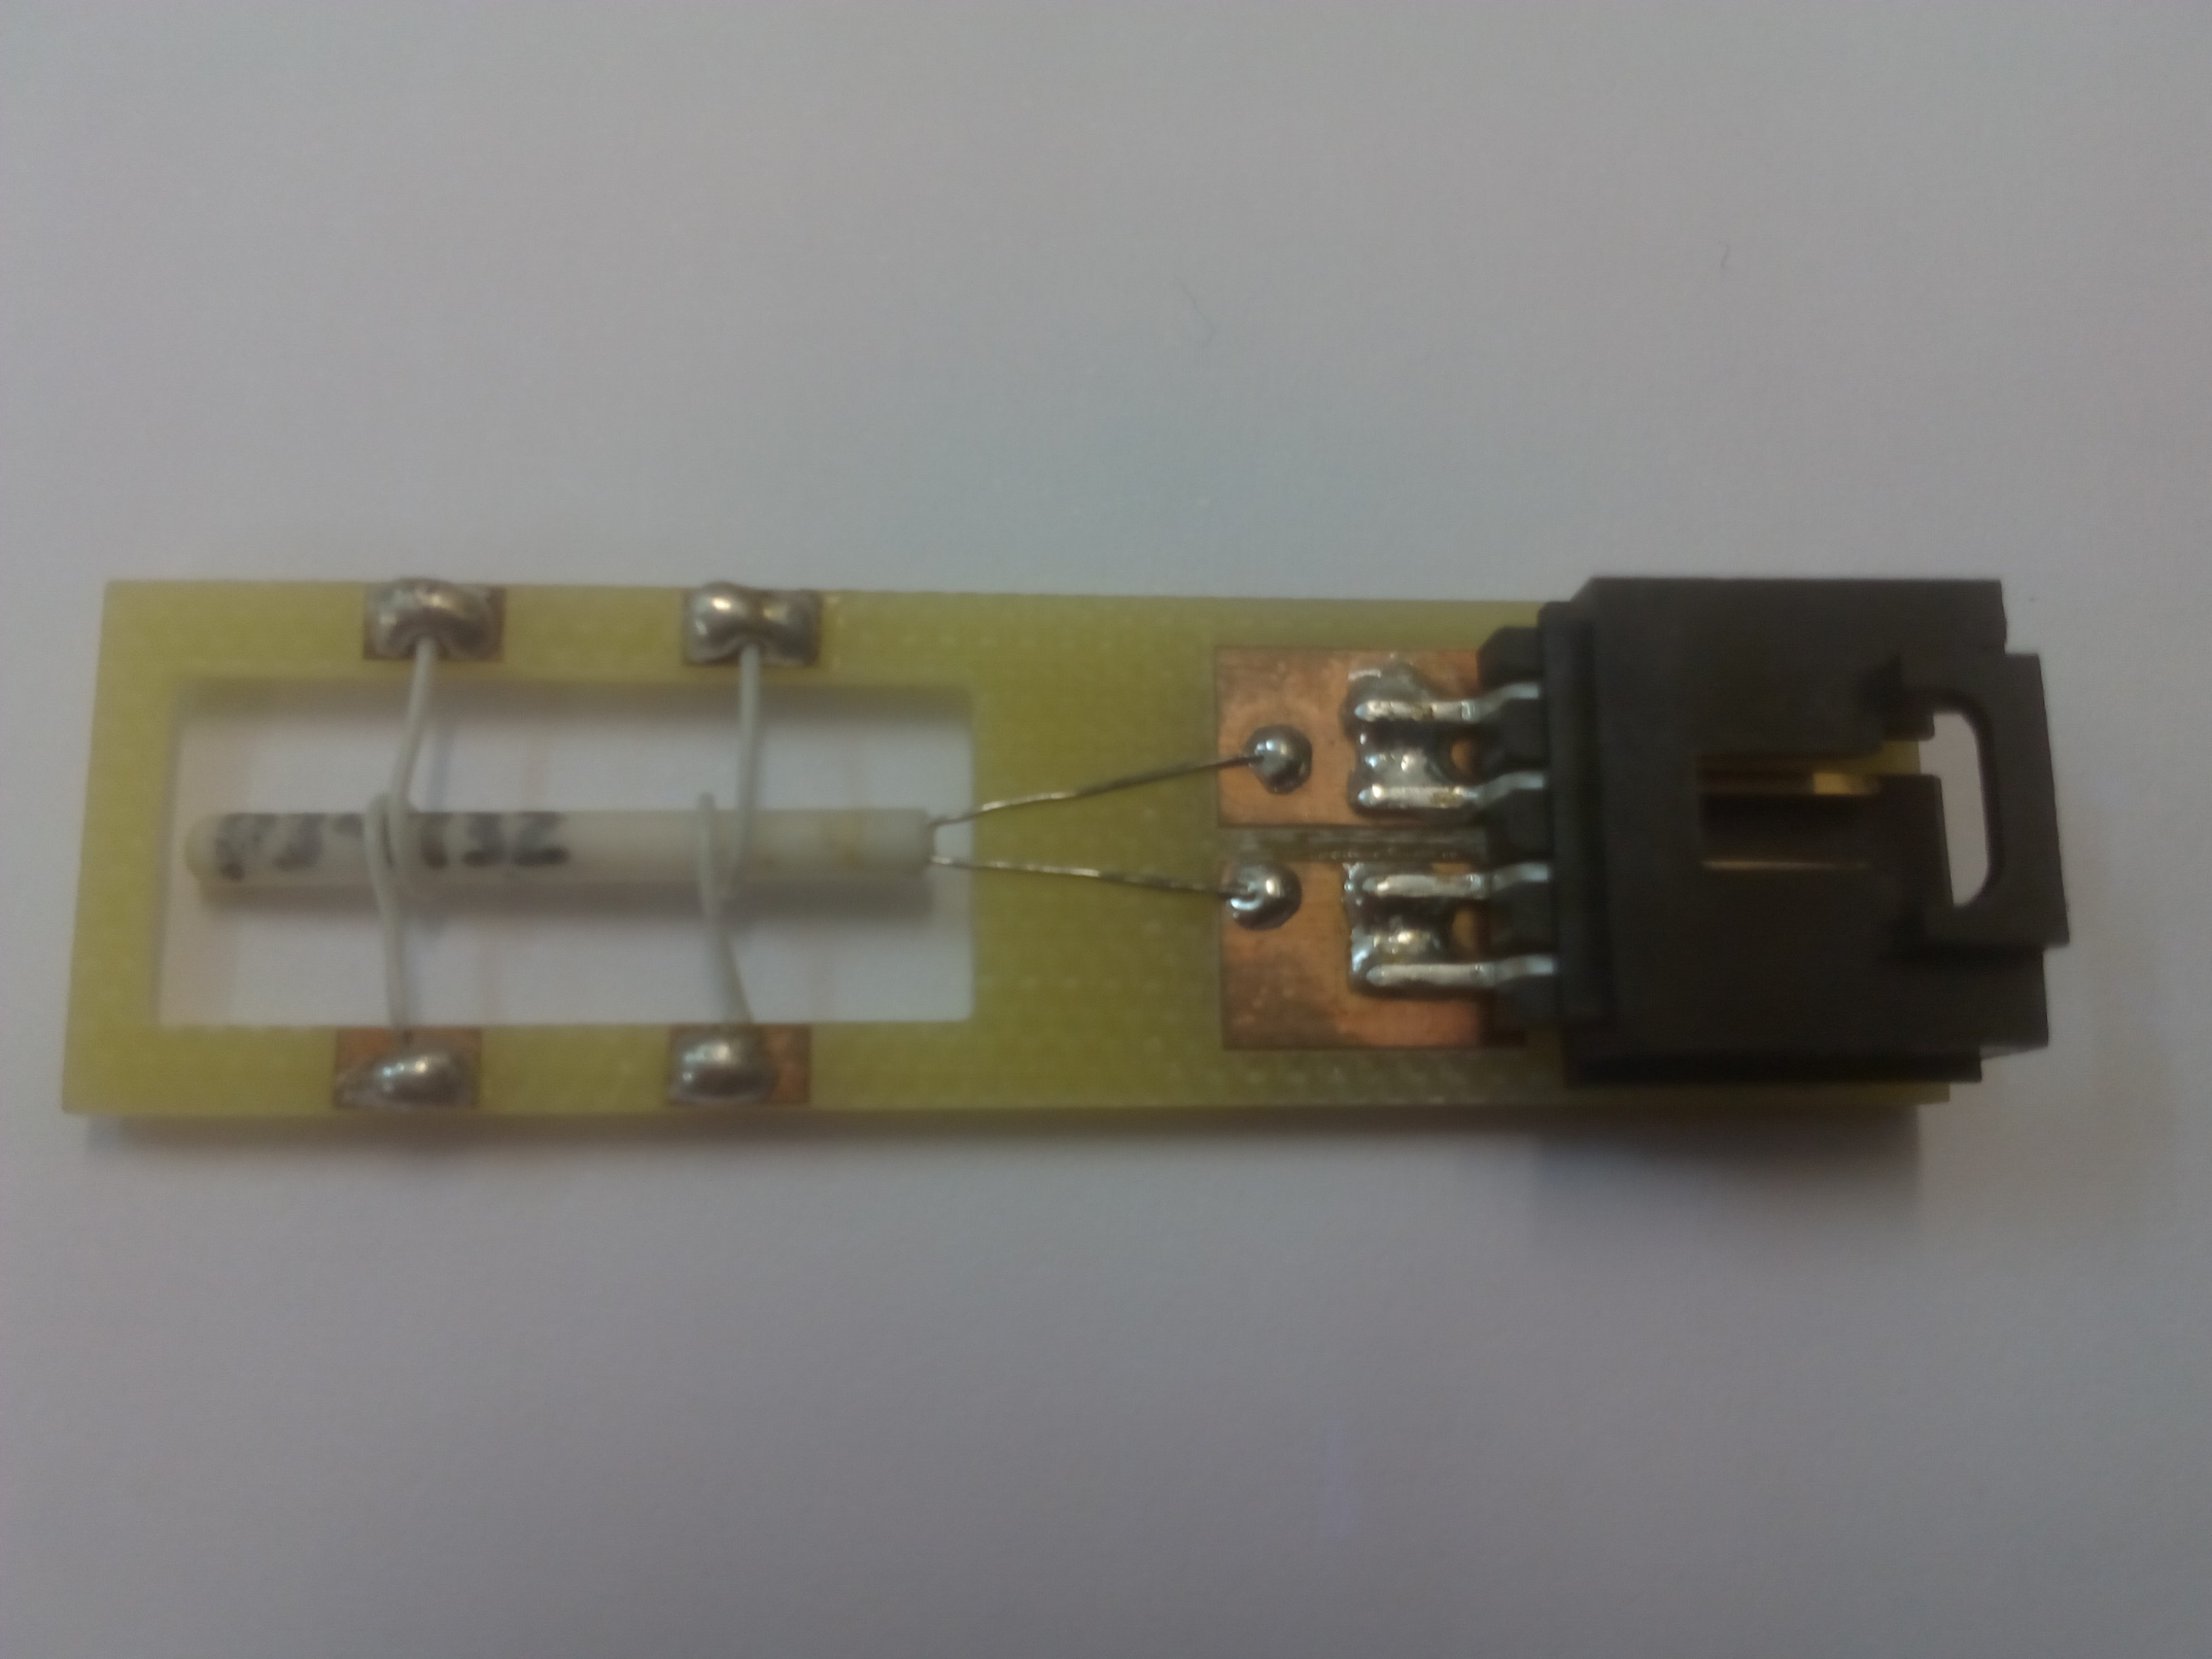
\includegraphics[width=0.3\textwidth]{sensor_support.jpg}%
\end{dunefigure}

% % % %
\subsubsection{Dynamic T-Gradient monitors}

% % % %
\subsubsection{Individual Temperature Sensors}

T-Gradient monitors will provide a vertical temperature profiling outside the TPCs. Those will be complemented by a coarser 2D array at the top and bottom of the
detector. Sensors, cables and readout will be the same as for the T-gradient monitors. 

In principle a similar distribution of sensors will be used at TOP and bottom.
Following ProtoDUNE-SP design, bottom sensors will use the cryogenic pipes as support structure, while top sensors will be anchored to the ground planes.
Teflon (see Fig.~\ref{fig:cable-support}) pieces will be used to route cables from the sensors to the DSS/cryogenic ports.


\begin{dunefigure}[sensorcable support]{fig:cable-support}
  {Left: support for two cables on ground planes. Right: Supports for three cables  mounted on cryogenics pipes using split clamps}
% This PDF is made from the .dot of the same name.
  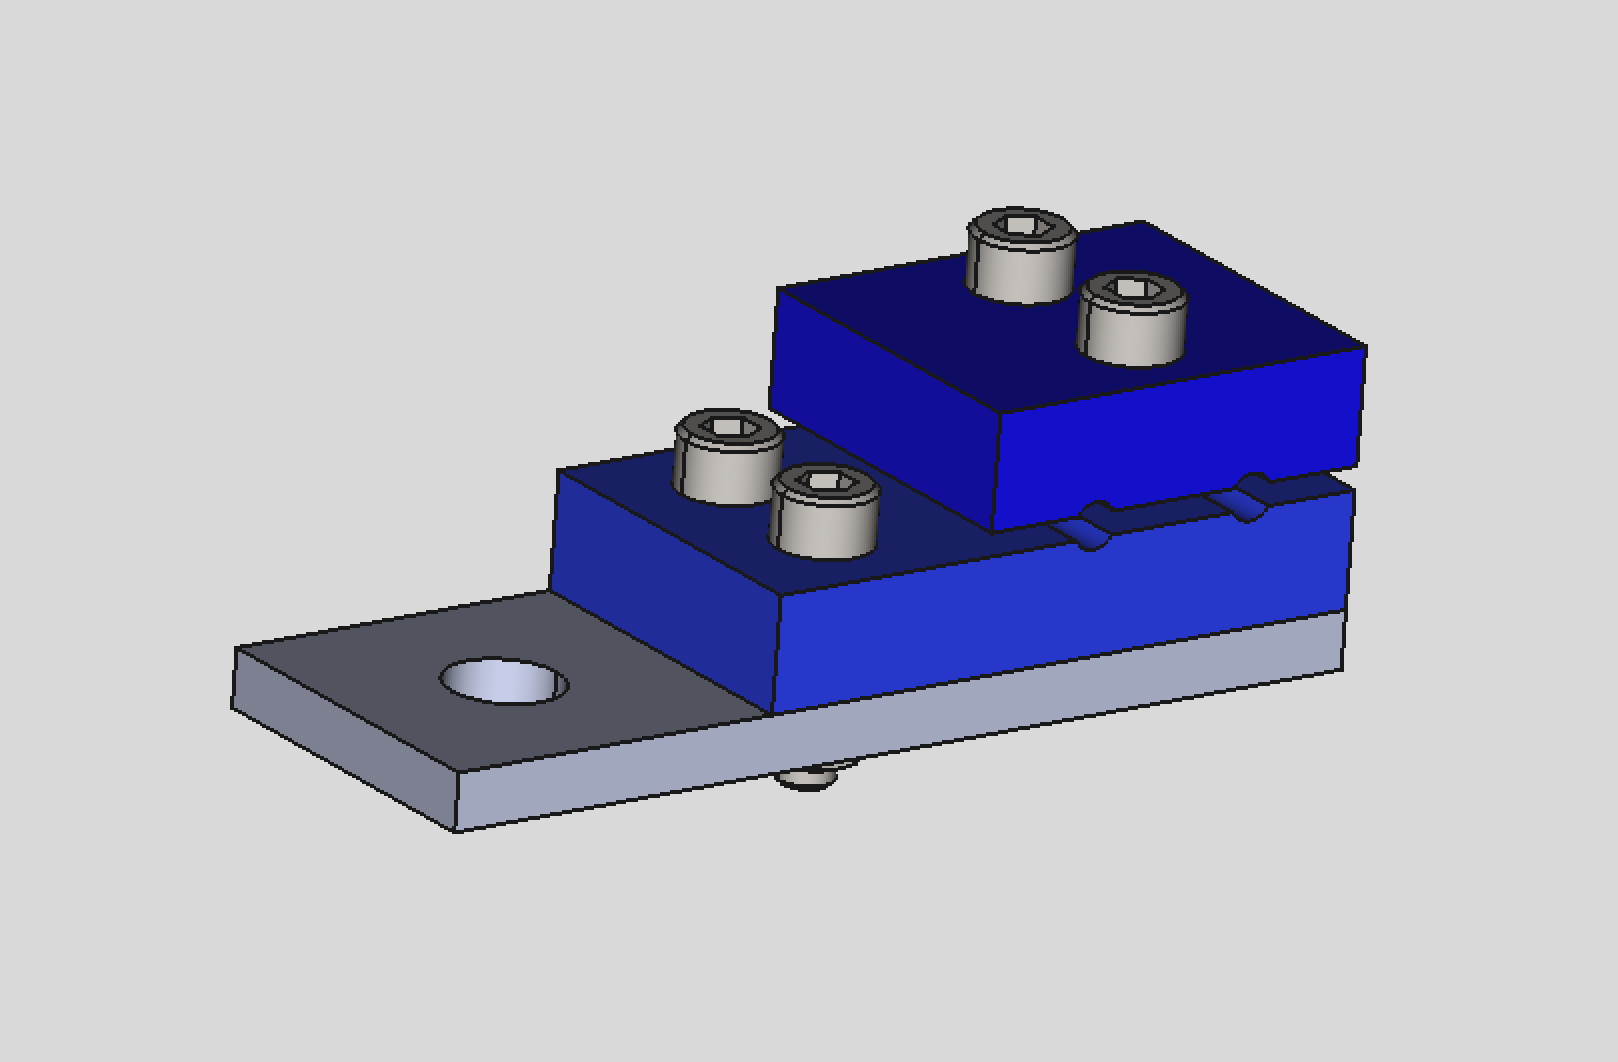
\includegraphics[width=0.3\textwidth]{cable_support_gp.png}
  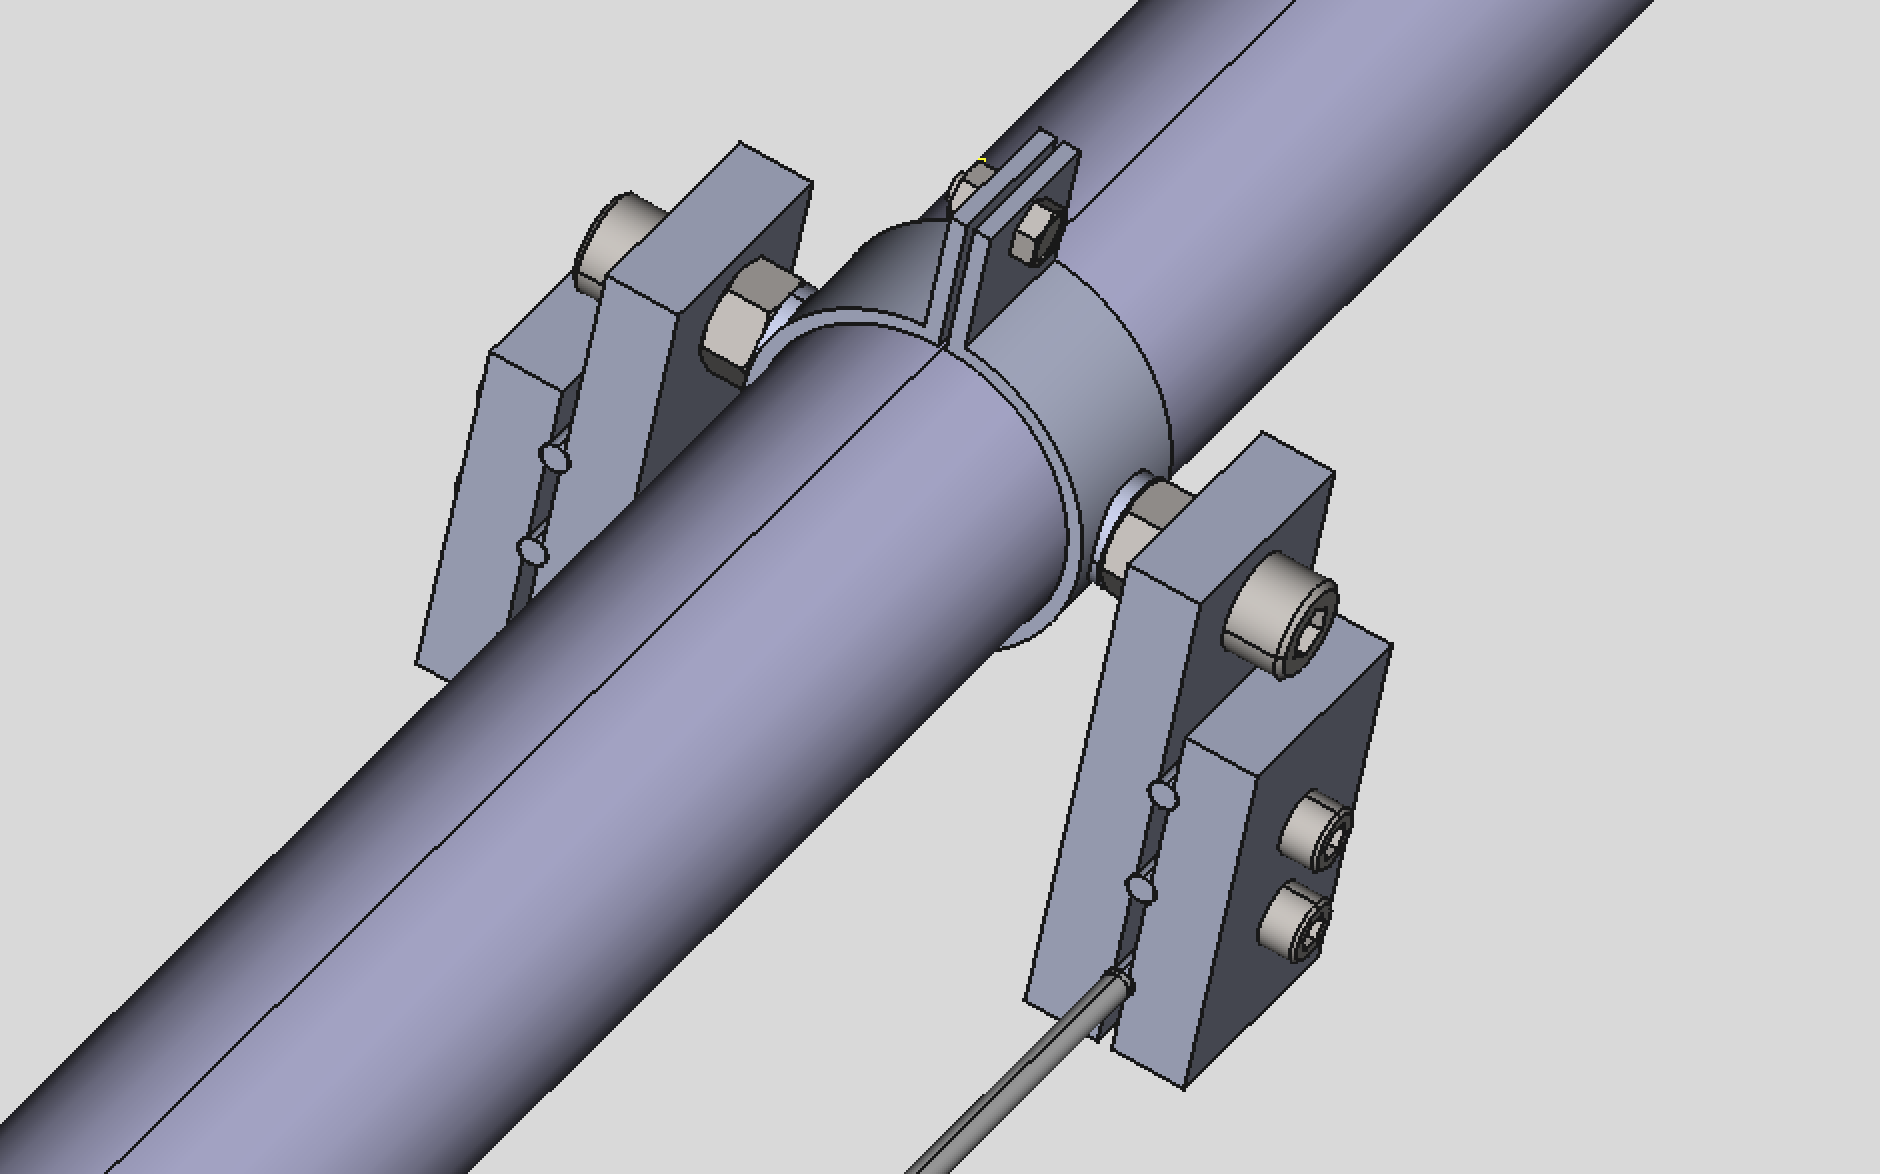
\includegraphics[width=0.315\textwidth]{cable_support_pipes.png}
\end{dunefigure}


% % % %
\subsubsection{Readout system for thermometers}
\label{sec:fdsp-slow-cryo-therm-readout}

A high precision and very stable system is required to achieved the design precission of $< 5 mk$.
The proposed readout system for the temperature sensors is based on a variant of an existing mass PT100 temperature readout system developed at CERN for one of the LHC experiments.
The goal of this system is to improve the precision as a reference system (Lakeshore 218) that the collaboration had evaluated as being appropriate,
but with reduced cost and space utilization.
The system consists of three parts:
\begin{itemize}
\item An accurate current source for the excitation of the temperature sensors, implemented by a compact electronic circuit using high a precision voltage reference from Texas Instruments. 
\item A multiplexing circuit based on an ADG707 Analog Device multiplexer electronic device;
\item A hig resolution and accuracy voltage signal readout module based on National Instruments NI9238, which has 24 bits resolution over 1 Volt range.
  This module is inserted in a National Instruments Ethernet DAQ backplane, which will distribute the temperature values to the main Slow Control Software
  through the standard protocol, OPC UA. The Ethernet DAQ will include also the multiplexing logic.
\end{itemize}
